% Cover letter using letter.sty
\documentclass[11pt]{letter} % Uses 10pt
%Use \documentstyle[newcent]{letter} for New Century Schoolbook postscript font
% the following commands control the margins:
\topmargin=-1in    % Make letterhead start about 1 inch from top of page
\textheight=10in  % text height can be bigger for a longer letter
\oddsidemargin=0pt % leftmargin is 1 inch
\textwidth=6.5in   % textwidth of 6.5in leaves 1 inch for right margin
\usepackage{wrapfig}
\usepackage{graphicx}
\begin{document}

\signature{Rapid Scheduling, Inc.}           % name for signature
\longindentation=0pt                       % needed to get closing flush left
\let\raggedleft\raggedright                % needed to get date flush left


\begin{letter}{Memo to:\\
United States Government\\
Department of the Big Long River}


\vfill % forces letterhead to top of page


\opening{To the Managers of the Big Long River,}

Rapid Scheduling Incorporated was thrilled to receive your request for our
optimization software. As a rapid scheduling company we are very familiar
with your type of request. We have taken the liberty of preparing a scheduling
program which will schedule all the visitors to your river with ease. Fear
not, it comes with an easy-to-use interface, sampled at the bottom right of
this letter.

\noindent
The scheduler is prepared to handle any type of request. This includes
each visitor's preferred boat type, departure date, and how long they'd
like to spend on the river each day. Naturally, visitors will have their
own campsite for each night they spend on the river. The program will even
calculate how satisfied your visitors will be at the end of their trip. A
visitor's estimated satisfaction will fall if they pass or are passed by
another group during their trip, if they spend more or less time on the
water than they desire, or if they cannot be scheduled.

\noindent
There are some constraints that you should be aware of before implementing
our software. We assume that campsites are evenly spaced along the river.
We also assume that visitors are willing to follow the schedule we assign
them. The software implements a tolerance for the distance each visitor
will travel every day. While exercising this tolerance does likely decrease the
satisfaction of a visitor, it also allows many more visitors to travel the
river each season.

\begin{wrapfigure}{r}{0.5\textwidth}
  \begin{center}
    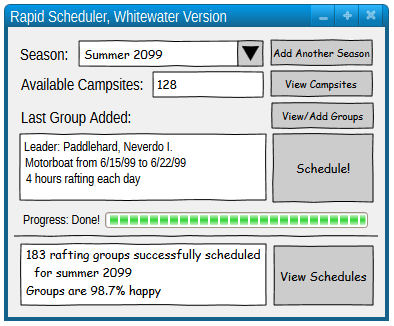
\includegraphics[width=0.45\textwidth]{sampleinterface.png}
  \end{center}
\end{wrapfigure}

\noindent
For instance, a 180 day season allowing visitors no
tolerance (they always travel the distance they want) might only allow 173
visitors per season, if they leave consecutively and all travel
the same speed. By increasing the tolerance to just two campsites per night,
however, it is quite possible to allow up to 300 visitors each season, for
entirely random speeds and departure dates.

\noindent
The software is capable of scheduling more than 600 visitors per season.
Their speeds, departure dates, and the amount of time they desire on the
river, however, may need to be very specific. With 600 visitors per season,
only about 5\% of completely random combinations will work.

\noindent
Your river is big and long, and it deserves to be appreciated by as many
visitors as possible.\\ Our software can help you do just that.


\noindent

\closing{Keep paddling,}



%\encl{ }  				% Enclosures
 \vfill
\end{letter}


\end{document}






